\documentclass[letterpaper]{article}

%%%%%%%%%%%%%%%%%%%%%%%%%%%%%%%%%%%%%%%%%%%%%%%%%
%%%%                  HI!                    %%%%
%%%%        THIS IS THE SSI-BIOLOGY			 %%%%
%%%%      GENERIC PROCEDURE TEMPLATE :) 	 %%%%
%%%%      IT MIGHT LOOK SCARY, BUT IT'S 	 %%%%
%%%%           PRETTY EASY TO USE 			 %%%%
%%%%%%%%%%%%%%%%%%%%%%%%%%%%%%%%%%%%%%%%%%%%%%%%%

%%%%%%%%%%%%%%%%%%%%%%%%%%%%%%%%%%%%%%%%%%%%%%%%%%%%%%%%%%
%%%%      RIGHT NOW YOU'RE LOOKING AT BOILERPLATE     %%%%
%%%%  THAT IS, THINGS YOU DON'T HAVE TO CHANGE (EVER) %%%%
%%%%     SCROLL DOWN FOR THE THINGS YOU SHOULD PAY    %%%%
%%%%    ATTENTION TO :)  (YOU'LL KNOW WHEN TO STOP)   %%%%
%%%%%%%%%%%%%%%%%%%%%%%%%%%%%%%%%%%%%%%%%%%%%%%%%%%%%%%%%%


%% Language and font encodings
\usepackage[english]{babel}
\usepackage[utf8x]{inputenc}
\usepackage[T1]{fontenc}

%% Sets page size, footer, indent and margins
\usepackage[a4paper,top=2.5cm,bottom=2.5cm,left=2.25cm,right=2.25cm,marginparwidth=2.25cm]{geometry}
\setlength\parindent{0pt}
\setlength{\footskip}{55pt}

%% Useful packages
\usepackage{amsmath}
\usepackage{graphicx}
\usepackage{fancyhdr}
\pagestyle{fancy}
\usepackage{textcomp}
\usepackage{gensymb}
\usepackage{hyperref}
\usepackage{readarray}
\usepackage{verbatimbox}
\usepackage{framed}
\usepackage[dvipsnames]{xcolor}
\usepackage{tcolorbox}
\usepackage{colortbl}
\usepackage{libertine} 
\usepackage{siunitx}
\usepackage{wrapfig}

% Safety Environment 
\definecolor{safetyFrame}{HTML}{FFFFFF}
\newenvironment{safety}{%
\begin{tcolorbox}[width=\textwidth, colframe=safetyFrame, arc=1.5mm]
}%
{\end{tcolorbox}}


% Footer
\lfoot{
\includegraphics[height=1.5cm]{1000x350-Horiz-Logo-WhiteRed-BlackText.png}}
\rfoot{
\includegraphics[height=1.25cm]{smol.png}}

% Substitution Commands
\newcommand{\tdt}{Terminal Deoxynucleotidyl Transferase}
\newcommand{\C}{\degree{}C}
\newcommand{\uL}{\micro{}L}
\newcommand{\BdATP}{3'-O-(2-nitrobenzyl)-2'-dATP}

%Custom Commands
\newcommand{\B}[1]{\textbf{#1}}

% Safety Info
\newcommand{\SYBRGOLD}{\item{\B{SYBR Gold} has no data available addressing the mutagenicity or toxicity of SYBR® Gold nucleic acid gel stain. Because this reagent binds to nucleic acids, it should be treated as a potential mutagen and handled with appropriate care. The DMSO stock solution should be handled with particular caution as DMSO is known to facilitate the entry of organic molecules into tissues.\cite{sybrGold}}}
\newcommand{\SYBRI}{\item{\B{SYBR Green I} is a mutagen and can penetrate laboratory gloves in a relatively short period of time, please change your gloves in the event of contamination. See \url{http://www.sigmaaldrich.com/MSDS/MSDS/DisplayMSDSPage.do?country=US&language=en&productNumber=S9430&brand=SIAL} for more information on the specifics of SYBR Green I. 
}}
\newcommand{\ETBR}{\item{\B{Ethidium Bromide} is a \B{serious mutagen} and is \B{significantly carcinogenic}. If working with considerable amounts, a \B{fume hood and respirator} are warranted. For more information see \url{https://www.sciencelab.com/msds.php?msdsId=9927667}
}}


% Shortcuts

%Stop Point (Optional)
\newcommand{\stopPoint}{\begin{center}
\rule{0.5\textwidth}{.4pt}\\
\vspace{1mm} 
OPTIONAL STOP POINT\\
\rule{0.5\textwidth}{.4pt}
\end{center}}

\newcommand{\RstopPoint}{\begin{center}
\rule{0.5\textwidth}{.4pt}\\
\vspace{1mm} 
RECOMMENEDED STOP POINT\\
\rule{0.5\textwidth}{.4pt}
\end{center}}

% Dilution Macro
\newcommand{\Dilution}[4]{
\subsection{#2}
\begin{enumerate}
\item{Vortex #2 stock}
\item{Pipette #1\uL{} #2 into a PCR Tube}
\item{Pipette #3\uL{} #4 into solution}
\item{Vortex until mixed}
%\item{Pipette $#2\mu L$ Water into solution}
\end{enumerate}
}

% Gel Macro
\newcommand{\gel}[4]{
\begin{figure}[ht]
\label{#2}
\begin{center}
\includegraphics[width=0.45\textwidth]{#1}
\caption{#2}
\end{center}
\subsection{#3 Analysis}
#4
\end{figure}
}

% Well plate Macro
\newcommand{\wellplate}[2]{
\getargsC{#1}
\begin{tabular}{*{1}{>{\columncolor{blue!20}}l}|l|l|l|l|l|l|l|l|l|l|l|l|}
\rowcolor{blue!20}%
 & 1  & 2  & 3  & 4  & 5  & 6 & 7 & 8 & 9 & 10 & 11 & 12\\ \hline
\ifdefined\argxii
A & \argi & \argii & \argiii & \argiv & \argv & \argvi & \argvii & \argviii & \argix & \argx & \argxi & \argxii \\ \hline\fi
\ifdefined\argxxiv
B & \argxiii & \argxiv & \argxv & \argxvi & \argxvii & \argxviii & \argxix & \argxx & \argxxi & \argxxii & \argxxiii & \argxxiv \\ \hline\fi
\ifdefined\argxxxvi
C & \argxxv & \argxxvi & \argxxvii & \argxxviii & \argxxix & \argxxx & \argxxxi & \argxxxii & \argxxxiii & \argxxxiv & \argxxxv & \argxxxvi \\ \hline\fi
\ifdefined\argxlviii
D & \argxxxvii & \argxxxviii & \argxxxix & \argxl & \argxli & \argxlii & \argxliii & \argxliv & \argxlv & \argxlvi & \argxlvii & \argxlviii \\ \hline\fi
\ifdefined\arglx
E & \argxlix & \argl & \argli & \arglii & \argliii & \argliv & \arglv & \arglvi & \arglvii & \arglviii & \arglix & \arglx \\ \hline\fi
\ifdefined\arglxxii
F & \arglxi & \arglxii & \arglxiii & \arglxiv & \arglxv & \arglxvi & \arglxvii & \arglxviii & \arglxix & \arglxx & \arglxxi & \arglxxii \\ \hline\fi
\ifdefined\arglxxxiv
G & \arglxxiii & \arglxxiv & \arglxxv & \arglxxvi & \arglxxvii & \arglxxviii & \arglxxix & \arglxxx & \arglxxxi & \arglxxxii & \arglxxxiii & \arglxxxiv \\ \hline\fi
\ifdefined\argxcvi
H & \arglxxxv & \arglxxxvi & \arglxxxvii & \arglxxxviii & \arglxxxix & \argxc & \argxci & \argxcii & \argxciii & \argxciv & \argxcv & \argxcvi \\ \hline\fi
\end{tabular}
}

\newcommand{\tdtSafety}{\item{\textbf{\tdt{}} is toxic if inhaled. May cause cancer. Toxic to aquatic life with long lasting effects. Avoid breathing dust/fume/gas/mist/vapours/spray. Use personal protective equipment as required. If Inhaled: Remove victim to fresh air and keep at rest in a position comfortable for breathing. Dispose of contents/container in accordance with local/regional/national/international regulations.\cite{Invitrogen2002}}}

\usepackage{enumitem,amssymb}
%%%%%%%%%%%%%%%%%%%%%%%%%%%%%%%%%%%%%%%%%%%%%%%
%%%%%%%%%%%%%%%%%%%%%%%%%%%%%%%%%%%%%%%%%%%%%%%
%%%%%%%%%%%%% End of Boiler Plate %%%%%%%%%%%%%
%%%%%%%%%%%%%%%%%%%%%%%%%%%%%%%%%%%%%%%%%%%%%%%
%%%%%%%%%%%%%%%%%%%%%%%%%%%%%%%%%%%%%%%%%%%%%%%

%%%%%%%%%%%%%%%%%%%%%%%%%%%%%%%%%%%%%%%%%%%%%%%
%%%%%   AKA YOU WRITE AFTER THIS POINT    %%%%%
%%%%%%%%%%%%%%%%%%%%%%%%%%%%%%%%%%%%%%%%%%%%%%%


\title{XCell Perfect Page I} % CHANGE THIS
\author{Written by \textbf{Alan Tomusiak}\\ % CHANGE THIS 
		Checked by \textbf{Michael Uttmark}\\%Checked by \textbf{}\\ % CHANGE THIS
        For the Stanford Student Space Initiative Biology Subteam}
\date{\textbf{Written:} October 16, 2017 \,\textbf{Performed:} October 18, 2017 \,\textbf{Printed:} \today{}}

\begin{document}

\maketitle
\section{Procedure Purpose} % CHANGE THIS
Empirically test the capabilities of the XCell Surelock Mini-Cell Electrophoresis system, specifically to determine whether DNA resolution on the scale of a single base pair is possible within one well. 

\section{Overview} % CHANGE THIS 
This lab will run oligonucleotides of different lengths on a polyacrylamide gel electrophoresis (PAGE) gel system. By re-creating an experimental procedure run previously (Perfect PAGE II \& III) on a different gel electrophoresis system, we can achieve a better sense of the capabilities provided by the XCell Surelock apparatus and its compatible 20\% polyacrylamide gels. The results of this experiment will inform future experiments relying on a reliable, simple, inexpensive and fast method for differentiating ssDNA strands differing by a single base pair. 

% Safety First! ALSO, % CHANGE THIS
\section{Safety Information}
\begin{safety}
\begin{enumerate}
\SYBRGOLD{} % For select reagents, I've created custom commands so we don't have to copy and paste every time :)
\item{Working in a communal lab space is dangerous. Do not assume your fellow workers cleaned up sufficiently}
\end{enumerate}
\end{safety}

\section{Materials}
\begin{enumerate}
\item{15-well 20\% polyacrylamide gel.}
\item{XCell Surelock Mini-Cell Electrophoresis System}
\item{Gel Loading Buffer II}
\item{100 uM 15 bp oligo}
\item{100 uM 16 bp oligo}
\item{100 uM 25 bp oligo}
\item{100 uM 26 bp oligo}
\item{100 uM 35 bp oligo}
\item{100 uM 36 bp oligo}
\item{10/60 Ladder}
\end{enumerate}
% Now for the _good_ stuff  
\section{Dilutions}
\begin{enumerate}
\item{15-Mer 40ng/\uL{} - Stock solution should have 457 nanograms of DNA per microliter. Pipette 44 \uL{} of stock primer into 456 \uL{} of water. Vortex and mix. Concentration is 40ng/\uL{} - label appropriately.}
\item{16-Mer 40ng/\uL{} - Stock solution should have 505 nanograms of DNA per microliter. Pipette 40 \uL{} of stock primer into 460 \uL{} of water. Vortex and mix. Concentration is 40ng/\uL{} - label appropriately.}
\item{25-Mer 40ng/\uL{} - Stock solution should have 761 nanograms of DNA per microliter. Pipette 26 \uL{} of stock primer into 474 \uL{} of water. Vortex and mix. Concentration is 40ng/\uL{} - label appropriately.}
\item{26-Mer 40ng/\uL{} - Stock solution should have 786 nanograms of DNA per microliter. Pipette 26 \uL{} of stock primer into 474 \uL{} of water. Vortex and mix. Concentration is 40ng/\uL{} - label appropriately.}
\item{35-Mer 40ng/\uL{} - Stock solution should have 1070 nanograms of DNA per microliter. Pipette 19 \uL{} of stock primer into 481 \uL{} of water. Vortex and mix. Concentration is 40ng/\uL{} - label appropriately.}
\item{36-Mer 40ng/\uL{} - Stock solution should have 1103 nanograms of DNA per microliter. Pipette 18 \uL{} of stock primer into 482 \uL{} of water. Vortex and mix. Concentration is 40ng/\uL{} - label appropriately.}
\item{Custom DNA Ladder 240ng/\uL{} - Add 44 \uL{} of 15-Mer stock, 40 \uL{} of 16-Mer stock, 26 \uL{} of 25-Mer stock, 26 \uL{} of 26-Mer stock, 19 \uL{} of 35-Mer stock, and 18 \uL{} of 36-Mer stock to 327 \uL{} of water. Concentration is 240ng/\uL{} - label appropriately. }
\item{15-Mer 8ng/\uL{} - Pipette 100\uL{} of the 15-Mer 40ng/\uL{} aliquot into 400\uL{} of water. Vortex and mix. Concentration is 8ng/\uL{} - label appropriately.}
\item{16-Mer 8ng/\uL{} - Pipette 100\uL{} of the 16-Mer 40ng/\uL{} aliquot into 400\uL{} of water. Vortex and mix. Concentration is 8ng/\uL{} - label appropriately.}
\item{25-Mer 8ng/\uL{} - Pipette 100\uL{} of the 25-Mer 40ng/\uL{} aliquot into 400\uL{} of water. Vortex and mix. Concentration is 8ng/\uL{} - label appropriately.}
\item{26-Mer 8ng/\uL{} - Pipette 100\uL{} of the 26-Mer 40ng/\uL{} aliquot into 400\uL{} of water. Vortex and mix. Concentration is 8ng/\uL{} - label appropriately.}
\item{35-Mer 8ng/\uL{} - Pipette 100\uL{} of the 35-Mer 40ng/\uL{} aliquot into 400\uL{} of water. Vortex and mix. Concentration is 8ng/\uL{} - label appropriately.}
\item{36-Mer 8ng/\uL{} - Pipette 100\uL{} of the 36-Mer 40ng/\uL{} aliquot into 400\uL{} of water. Vortex and mix. Concentration is 8ng/\uL{} - label appropriately.}
\item{Custom DNA Ladder 48 ng/\uL{} - Pipette 100\uL{} of the Custom DNA Ladder 240ng/\uL{} aliquot into 400\uL{} of water. Concentration is 48ng/\uL{} - label appropriately. }
\end{enumerate}
\section{Procedure}% CHANGE THIS
\textbf{Note} In case there are many participants in this experiment, a second gel can be run using half as much volume in each well. This has been suggested to provide cleaner gel readings.
\begin{enumerate} 
\subsection{Sample Preparation}
\item{Complete all dilutions and ensure all are appropriately labeled and well mixed.}
\stopPoint{} 
\item{Let Gel Loading Buffer II and 10/60 Oligo Ladder thaw.}
\subsection{XCell Surelock Setup and Pre-Run}
\item{Remove 20\% polyacrylamide gel from pouch and rinse with deionized water.}
\item{Peel off tape on bottom of 20\% polyacrylamide gel and remove the comb.}
\item{Gently wash every cassette well with 1X TBE buffer. Invert to remove buffer and shake. Repeat twice.}
\item{Lower the Buffer Core (the piece that holds the gels) into the Lower Buffer Chamber so that the negative electrode fits into the opening in the gold plate.}
\item{Insert the Gel Tension Wedge into the XCell Surelock behind the buffer core. Make sure it is in its 'unlocked' position, which allows the wedge to slip into the unit.}
\item{Insert gel cassettes into the lower buffer chamber. The shorter "well" side of the cassette faces into the buffer core. The slot on the back must face outward. If only one gel is being run, insert a buffer dam in the place of a gel cassette.}
\item{Pull forward on the Gel Tension Lever toward the buffer core until the gel cassettes are snug against the buffer core. This puts it in the 'locked' position.}
\item{Fill the Upper Buffer Chamber (between the gels) with running buffer. Ensure it is not leaking.}
\item{Fill the Lower Buffer Chamber completely with running buffer by pouring TBE next to the Gel Tension Wedge.}
\item{Pipette 12\uL{} of running buffer into each gel well.}
\item{Place the gel cover on the apparatus in the correct orientation. Connect the electrodes to the power source, and pre-run the gel for 30 minutes at 150V.}


\subsection{Gel Loading and Running}
\begin{figure}[ht] %This is a figure, in this case, a well plate
\begin{center} 
\addvbuffer[{0mm} \baselineskip]{\begin{tabular}{|l|l|}
\hline
Well number    & Sample \\ \hline
1                                  & 10/60 DNA Ladder   \\ \hline
2								   & 15-Mer (40 ng) \\ \hline
3                                  & 16-Mer (40 ng) \\ \hline
4                                  & 25-Mer (40 ng) \\ \hline
5                                  & 26-Mer (40 ng)  \\ \hline
6								   & 35-Mer (40 ng) \\ \hline
7                                  & 36-Mer (40 ng)  \\ \hline
8                                  & Custom DNA Ladder (240 ng)   \\ \hline
9                                  & 10/60 DNA Ladder  \\ \hline
10                                  & Blank \\ \hline
11                                  & 15-Mer (40ng) \\ \hline
12                                 & 16-Mer (40ng)     \\ \hline
13                                 & Blank      \\ \hline
14                                 & Custom DNA Ladder (240 ng)  \\ \hline
15								   & 10/60 DNA Ladder \\ \hline

\end{tabular}}
\label{tab:Gel Layout} %Label your stuff, this is for referencing in the future
\caption{Wells} %Caption!
\end{center}
\end{figure}
\textbf{Note} Be relatively swift about mixing and loading, as the samples will gradually begin to evaporate if left on the parafilm for too long.
\item{Obtain a sizable piece of parafilm. Pipette 5 \uL{} of Gel Loading Buffer in a row of 15 droplets.}
\item{In the first and fourteenth droplet, pipette 1uL of 15/60 Ladder and 4 uL of TBE loading buffer and mix. For the 'blank' droplets, pipette 5uL of running buffer.}
\item{For the remaining droplets, add 5 \uL{} of the appropriate sample. See the corresponding table for sample location and order.}
\item{As you go, pipette up and down to mix thoroughly.}
\item{Load the gels (with 10 \uL{} sample in each well) when they are finished pre-running. Ensure pipette tip is fully in the well, and depress slowly and carefully. Work quickly to minimize diffusion.}
\item{If running a second gel, repeat steps 15-18, then pipette only 5uL of each sample into each well.}
\item{Run the gel(s) at 150V until the dark blue dye is 1cm from the bottom. If the dark blue dye is not visible, run the gel for two and a half hours.}
\end{enumerate}

\subsection{Staining and Viewing Gel}
\begin{enumerate}
\item{While the gel runs, prepare 1X SYBR Gold Staining Solution with TBE as dilute}
\item{Once gel has finished running, \textbf{\textit{lightly}} agitate gel while submerged in solution for 45 minutes.}
\item{Review gel with gel viewer. Until unnecessary, place gel back in stain for 20 minute increments and re-image.}
\item{Post pictures to Slack.}\\
\end{enumerate} 
% Stop Procedure
\section{Stop Procedure}
\begin{enumerate}
\item{Place all samples back in the freezer. Absolutely ensure that the SYBR Gold has been returned. Dispose of gels in the trash and TBE in the sink. Rinse the XCell Surelock system with deionized water and a mild detergent.}
\end{enumerate}

% * <tomusiak@stanford.edu> 2017-10-20T01:51:41.877Z:
%
% ^.
\section{Analysis}
\begin{figure}[ht]
\begin{center}
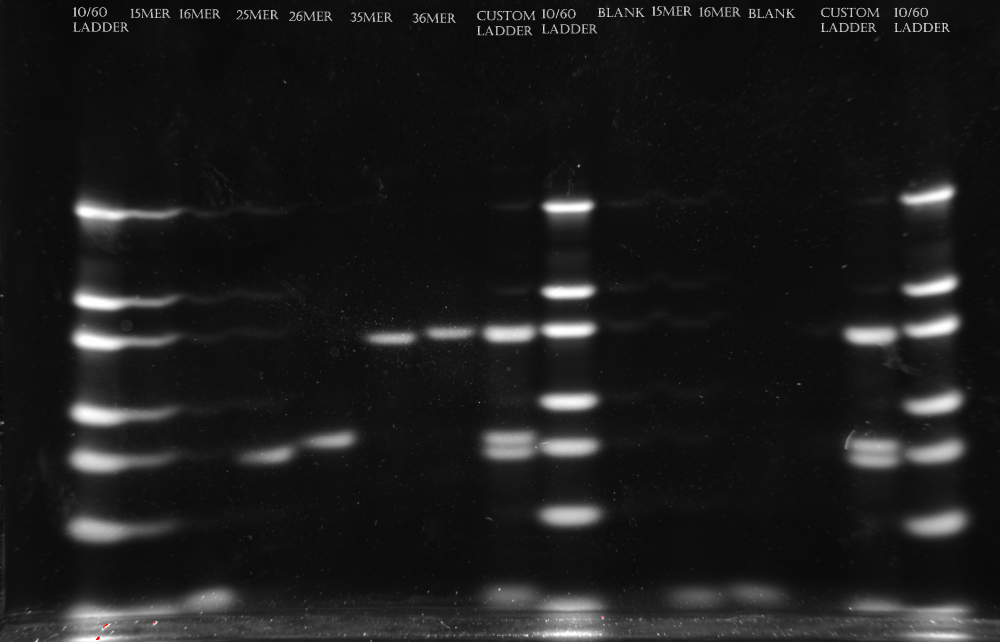
\includegraphics[width=.8\textwidth]{Alan_Ladder.png}
\caption{Gel 1}
\label{gels1}
\end{center}
\end{figure}
\begin{figure}[ht]
\begin{center}
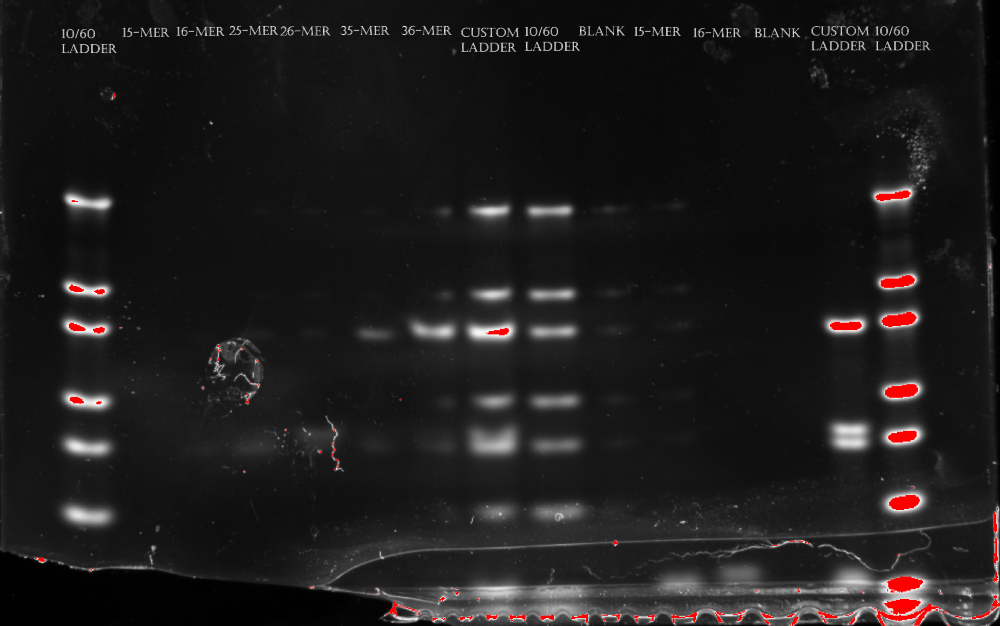
\includegraphics[width=.8\textwidth]{JacklynRyan_Gel.png}
\caption{Gel 2}
\end{center}
\end{figure}
\subsection{Experimental Notes}
\begin{enumerate}
\item{Two identical gels were run in an identical manner. Gel 1 was loaded before Gel 2. A significant period of time elapsed between the loading of Gel 1 and the beginning of the gel run.}
\item{The gel comb on Gel 1 was removed unevenly, resulting in tearing on the first three lanes and cross-contamination of sample.}
\item{Concern about sample overflow resulted in almost all of the samples being run at 5 \uL{} instead of the specified 10 \uL{}. This resulted in half of the specified nanogram amount of DNA being loaded in each lane, but each sample is still clearly visible.}
\item{A different power supply was utilized, as the Bio-Rad power supplies are incompatible with the XCell Surelock gel electrophoresis system.}
\item{Gel 2 had some issues with regarding to loading, resulting in what appeared to be 'breaking' of the well near well 5. This may have resulted in the lack of visible DNA bands.}
\item{Both gels were run until the dark blue dye was approximately half of a centimeter from the bottom of the gel apparatus.}
\end{enumerate}

\subsection{Experimental Results}
\begin{wrapfigure}{r}{0.15\textwidth}
\centering
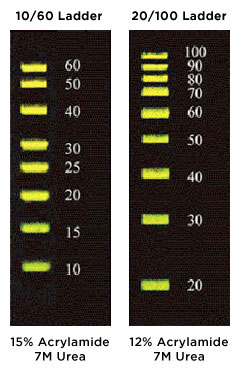
\includegraphics[height=1.5in]{1060_Ladder.jpg}
\caption{Ideal Ladder}
\label{Ideal Ladder}
\end{wrapfigure}
On both of the gels, the lack of a distinctive 15/16-mer band with clear brightness at the very bottom of the gel suggests that the two bands had run off the gel, rendering attempted single base-pair resolution impossible. However, in Gel 1, there are two different banding patterns for the 25-mer and the 26-mer in adjacent wells, although the 35-mer and 36-mer still appear to be indistinct. \\

On both Gel 1 and Gel 2, looking primarily at the 'Custom DNA Ladder' prepared by combining 15/16/25/26/35/36-mers, there appears to be clear separation between the 25-mer and the 26-mer, evidenced by comparison with the commercial Integrated DNA Technologies 10/16 ladder, where the two lanes appear to directly correspond to the '25 length' on the commercial ladder. This same result is replicated three times - twice on Gel 1 and once on Gel 2, suggesting that the custom ladder consistently separates 25-mers and 26-mers in the same lane. In every instance that 25-mers and 26-mers were run as part of the custom DNA ladder, the PAGE gel effectively separated the two strands.
\subsection{Conclusions}
It appears that it is possible to obtain single base-pair resolution in the same lane on a 20\% polyacrylamide gel using an XCell Surelock gel apparatus. This may be the result of the increased size of XCell pre-cast gels (rough a centimeter and a half longer than Bio-Rad pre-cast gels) and the increased polyacrylamide content of the gel itself. This capacity is significant for any synthesis method developed, as the ability to differentiate between two DNA segments one length apart provides not only a qualitative tool through which to investigate possible successful addition but also provides a rough quantitative functionality.
\\
\\
Experimentally, it may be wise to run the gel at 200 volts and wait until the dark blue stain reaches an inch from the bottom, as the setup of this experiment proved to be time-costly and resulted in the loss of valuable sample. The ability to differentiate between 25 and 26 base-pair long ssDNA strands was not expected nor hoped for, and provided a surprisingly positive result where one could have been lost due to running the sample off of the gel. However, this experiment also suggests that single base-pair resolution in the same lane can be achieved if the sample runs approximately 75\% down the length of the gel, meaning there is less risk in being cautious and stopping the gel early.

\bibliographystyle{ieeetr}
\bibliography{biblio}
\end{document}